\chapter{アンカーの発話の音声認識実験}
\label{chapter:speech_recog}
\subsection{音声認識システムの流れ}
音声認識の流れを図\ref{fig:flow_sp}に示す。まず、入力された音声データから前処理として雑音区間と無音区間を除去し、発話区間を検出する。次に検出した発話区間の音響的特徴量を抽出し、デコーダへと渡す。デコーダではこの音響的特徴量をもとに、音響モデルと言語モデル、単語辞書を参照しながら単語列の尤度を算出し、最も尤度の高いものを認識結果として出力する。言語モデルと単語辞書については\ref{language_model}節、音響モデルについては\ref{acoustic_model}節で説明する。

\begin{figure}[htb]
  \begin{center}
    \includegraphics{../../image/flow_sp.eps}
  \end{center}
  \caption{音声認識の流れ}
  \label{fig:flow_sp}
\end{figure}

\subsection{単語辞書と言語モデル}
\label{language_model}

\noindent{\textbf{\underline{単語辞書}}}\par
単語辞書には、一般的に学習データに出現する単語のなかで出現頻度の高い単語を登録する[7]。言語モデルもその単語辞書に登録された単語を用いて構築する。単語辞書の例を表\ref{table:tango}に示す。単語辞書には表記、発音形、原型、品詞番号、出現表記、音素表記などを登録する。\par

\begin{table}[htb]
  \begin{center}
    \caption{単語辞書の例}
    \begin{tabular}{|c||c|c|} \hline
      表記+発音形+原形+品詞番号 & 出力表記 & 音素表記 \\ \hline
      あか+アカ+アカ+14 & あか & a k a \\ \hline
      技術+ギジュツ+ギジュツ+1 & 技術 & g i zh j u ts u \\ \hline
      新聞+シンブン+シンブン+1 & 新聞 & sh i ng b u ng \\ \hline
    \end{tabular}
    \label{table:tango}
  \end{center}
\end{table}

音声認識では、言語モデルは、「表記+発音形+原型+品詞番号」を、音響モデルは「音素表記」の部分を用いて最尤の単語を算出する。辞書に登録している単語が少ない場合、入力された単語が辞書に登録されていないことが多くなり、他の誤った単語を出力し認識率が低下してしまう。一方、辞書に登録している単語が多すぎる場合、認識処理に時間がかかるだけでなく、認識候補が増えるため認識率が低下してしまう。よって適切な単語の登録数を検討する必要がある。

\noindent{\textbf{\underline{言語モデル}}}\par
音声認識における言語モデルとは、文の品詞や単語と単語の関係性、音素の並びの制約などを定式化したもののことである。言語モデルの主流はサンプルデータから統計的な手法によって確率推定を行なう統計的言語モデルである。その中でも最も広く使われているのが$N$グラムモデルである。\par
\noindent{\textbf{\underline{$N$グラムモデル}}}\par
$N$グラムモデルとは、与えられた単語列$\omega_1,\omega_2,\cdots,\omega_n$に対して、その出現確率$p(\omega_1,\omega_2,\cdots,\omega_n)$を推定する場合に、

\begin{equation}
P(\omega_1,\omega_2,\cdots,\omega_n)=\prod_{i=1}^{n}p(\omega_{i}\mid \omega_{i-N+1}\cdots \omega_{i-1})
\end{equation}

のような近似を行なうモデルである。$N$グラムモデルでは、$i$番目の単語$ω_i$の生成確率が、直前の$N-1$単語$ω_{i-N+1}\cdots ω_{i-2}ω_{i-1}$だけに依存すると考える。特に$N = 1$のときユニグラム(unigram)、$N = 2$のときバイグラム(bigram)、$N = 3$のときトライグラム(trigram)という。\par
文や発話中の単語の生成確率は文脈に依存することから、$N$グラムモデルの推定確率は、$N$が大きいほど高くなる。しかし、$N$グラムモデルは語彙の$N$乗のコストがかかることから、$N$を大きくするためには、膨大な量のテキストを用意しなければならない。しかし、自由発話を記述したテキストは極めて少ない。本研究では、$N = 3$のtrigramを用いる。\par



\subsection{音響モデル}
\label{acoustic_model}
音響モデルとは、音声の最小単位である音素または、単語や音節の音響特徴パラメータの時系列をモデル化したものである。この音素の特徴は、発話者や発話内容などによって変化するが、発話者ごと、または発話タスクごとにモデル化することは、膨大なコストがかかり汎用性がないため好ましくない。そのため、音響モデルの構築方法としては、音素ごとに様々な学習音声で学習を繰り返し、最尤の音響モデルを作ることが一般的である。本研究では、隠れマルコフモデル(Hidden Markov Model)を用いて最尤の音響モデルを構築する。\par
以下に音響モデルを構築する際に、必要となる知識について述べる。\par


\noindent{\textbf{\underline{MFCC}}}\par
メル周波数ケプストラム係数(Mel - Frequency Cepstrum Coefficient : MFCC)とは、メル周波数という人間の音の高低に対する感覚尺度で音声スペクトルから係数スペクトルを抽出したものである[7]。これは一般的に、音声の特徴を抽出するパラメータとして用いられる。
 MFCCの計算では、スペクトル分析は周波数軸上に$L$個の三角窓を配置し、フィルタバンク分析により行なう。すなわち、窓の幅に対応する周波数帯域の信号のパワーを、単一スペクトルチャネルの振幅スペクトル $|S^\prime (k)|$ の重み付けの和$m(l)$ で求める。

\begin{equation}
m(l)=\sum_{k=lo}^{hi}W(k;l)\mid S^\prime(k)\mid \quad (l=1,\cdots,L)
\end{equation}

\begin{equation}
W(k;l)=\begin{cases}\frac{k-k_{lo}(l)}{k_c(l)-k_{lo}(l)}\quad \{k_{lo}\leq k \leq k_c(l)\} \\\frac{k_hi(l)-k}{k_{hi}(l)-k_{l}(l)}\quad \{k_{c}\leq k \leq k_{hi}(l)\} \end{cases}
\end{equation}

ただし、$W(k;l)$ は重み、$k_{lo}(l)、k_c(l)、k_{hi}(l)$ はそれぞれ$l$番目のフィルタの下限、中心、上限のスペクトルチャネル番号であり、隣り合うフィルタ間で

\begin{equation}
k_c=k_{hi}(l-1)=k_{lo}(l+1)
\end{equation}

なる関係がある。さらに、$k_c(l)$はメル周波数軸上で等間隔に配置される。メル周波数は

\begin{equation}
Mel(f)=2595\log_{10}(1+\frac{f}{700})
\end{equation}

により計算される。ただし、$f$の単位は[Hz]にとる。\par
最終的にフィルタバンク分析により得られた$L$個の帯域におけるパワースペクトルを離散コサイン変換することで、式(\ref{eq:mfcc})のようにMFCCが得られる。

\begin{equation}
\label{eq:mfcc}
c_{mfcc}(i)=\sqrt{\frac{2}{N}}\sum_{i=1}^{L}\log ml \cos \left\{ \left( l-\frac{1}{2}\frac{i\pi}{L} \right)\right\}
\end{equation}


\noindent{{\textbf{\underline{隠れマルコフモデル(HMM)}}}\par
\noindent{{\textbf{\underline{調音結合}}}\par

\subsection{DNNの概要}

\section{実験方法}
本実験では、\ref{section:yoshimura_pre_clustering}節で述べる木構造話者クラスタを作成し、話者クラスタに含まれる学習データを用いて音響モデルを学習して音声認識実験を行う。各話者クラスタに含まれる男女の発話データ数を図\ref{fig:yoshimura_kikouzou}に示す。


\begin{figure}[H]
  \begin{center}
    \includegraphics[scale=0.5]{./figure/yoshimura.eps}
  \end{center}
  \caption{各話者クラスタに含まれる発話データ数 \label{fig:yoshimura_kikouzou}}
\end{figure}

学習データに用いた話者のi-vectorと認識するアンカーの発話のi-vectorのコサイン類似度を求め、求めたコサイン類似度の高い上位5人の学習データを全て含んでいるクラスタを選択し、選択したクラスタに含まれる学習音声で学習された音響モデルを用いて音声認識を行う。音響モデルの選択に用いるi-vectorと認識するアンカーの発話区間は\ref{chapter:get_anchor}節で検出したアンカーの発話区間のうち、各手法でもっともF値の高い条件のものを用いる。\par

本実験で使用した音響モデル、言語モデル、単語辞書の仕様は\ref{section:experiment_acoustic_model}節、\ref{section:experiment_language_model}節で述べる。

\section{音響モデルの仕様}
\label{section:experiment_acoustic_model}
本実験で用いたDNN-HMM音響モデルの仕様を表\ref{table:acoustic_model_detail}に示す。この仕様に関しては小島らの研究\cite{kojima}で使用されたもので、状態数は3000、音響特徴の次元数は39次元(表\ref{acoustic_model_feature})、隠れ層の数は6層、各層における繰り返し学習数は5回、隠れ層のノード数は1024とした。以下に、DNNを用いた際の学習の手順を示す。

\begin{table}[H]
  \begin{center}
    \caption{音響モデルの仕様 \label{table:acoustic_model_detail}}
    \begin{tabular}{|c|c|c|} \hline
     状態数  & 使用した音素 & 混合数 \\ \hline
     3,000  & 27 & 16 \\ \hline
    \end{tabular}
  \end{center}
\end{table}

\begin{table}[H]
  \begin{center}
    \caption{使用する音響特徴パラメータ \label{acoustic_model_feature}}
    \begin{tabular}{|c||c|} \hline
      特徴量 & 次元数\\ \hline
      MFCC & 12  \\ \hline
      POW & 1  \\ \hline
      $\Delta$MFCC & 12 \\ \hline
      $\Delta$POW & 1 \\ \hline
      $\Delta\Delta$MFCC & 12 \\ \hline
      $\Delta\Delta$POW & 1 \\ \hline
      計 & 39 \\ \hline
    \end{tabular}
  \end{center}
\end{table}



\vspace{0.2in}\noindent{\textbf{\underline{使用した音素}}}\par
本研究で使用した音素27個を表\ref{fig:used_onso}に示す。また、その音素をもとに記したカナ音素対応表を表\ref{fig:kana_onso}に示す


\begin{table}[H]
\begin{center}
\caption{使用した音素 \label{fig:used_onso}}
\begin{tabular}{|c|c|c|c|c|c|c|}
\hline
母音  & 子音         & 濁音  & 半濁音 & 撥音 & 促音 & 無音 \\ \hline
a i & ch f h j k & b d &     &    &    &    \\ 
u e & m n r s sh & g z & p   & ng & q  & \# \\ 
o   & t ts w     & zh  &     &    &    &    \\ \hline
\end{tabular}
\end{center}
\end{table}


\begin{table}[H]
  \begin{center}
    \caption{カナ音素対応表 \label{fig:kana_onso}}
    \includegraphics[scale=0.7]{./figure/kana_onso.eps}
  \end{center}
  
\end{table}

\section{i-vectorを用いた音声認識手法\cite{yoshimura_clustering}}
\label{section:yoshimura_pre_clustering}
学習データに含まれる話者の音響特徴を考慮して木構造話者クラスタを作成し、各話者クラスタに含まれる学習データを用いて音響モデルを学習した。この木構造話者クラスタは、母音の定常状態であるHMMの中央の状態の平均と分散を用いたBhattacharyya距離によるk-means法によって作成した。クラスタの個数は、最上位のクラスタを2分割し、作成された2つのクラスタをさらに2分割した計7つのクラスタを使用する。\par
認識の際は、学習データに用いた話者のi-vectorと評価データのi-vectorのコサイン類似度を求める。求めたコサイン類似度の高い上位$n$人の学習データを全て含んでいるクラスタを選択し、選択したクラスタに含まれる学習データで学習した音響モデルを用いて音声認識を行なった。\par

\section{言語モデル・単語辞書の仕様}
\label{section:experiment_language_model}
言語モデルはトライグラムモデルを構築した。以下、使用した学習テキストを説明する。

\vspace{0.2in}\noindent{\textbf{\underline{CSJ}}}\par
CSJには書き起こしテキストも提供されており、その一部の例を図\ref{fig:kakiokosi}に示す。書き起こしテキストは主に情報部と発話部に区別される。情報部では発話IDや時間情報等を、発話部では発話内容を「&」の左側に基本形、右側に発音形という形式で記している。発話形はカタカナを用いて実際に発音された音声を忠実に表記したものである。発音の怠けや言い間違い等を書き取れる範囲で忠実に記録している。本研究では、音響モデル構築の際には主に発話部の発音形を用い、このカタカナ表記を音素列に変換し、ラベルファイルとして定義する。
\begin{figure}[H]
  \begin{center}
    \includegraphics{./figure/kakiokosi.eps}
  \end{center}
  \caption{書き起こしテキストの例 \label{fig:kakiokosi}}
\end{figure}

本研究ではこのCSJをベースに学習テキストを構成する。使用するデータは977講演分のテキストで、約14MBである。

\vspace{0.2in}\noindent{\textbf{\underline{拡張したコーパスによる学習テキスト}}}\par
この学習テキストは江頭らによる、学術講演の書き起こしと新聞記事に拡張されるテキストとして参加者名の入ったテキスト、Webから収集してきたテキスト、そして対話コーパスから作成される対話テキストを追加した未知語の減少に着目した学習テキストである。この学習テキストは会議中に参加者の名前を呼ぶことが多い、会議は対話形式であるなどの会議の特徴を考慮した学習テキストである。テキストサイズは約100MBである。以降本論文では、このテキストを拡張したコーパスによる学習テキストと呼ぶ。

\vspace{0.2in}\noindent{\textbf{\underline{拡張したコーパスによる学習テキスト}}}\par
この学習テキストは荒井らによる、会議における発話行為に着目して作成された学習テキストである。学術講演の書き起こしと新聞記事に対話表現に近い特徴を持っていると考えられるQ&Aサイトから収集したテキストと対話コーパスを追加した学習テキストである。テキストサイズは約44MBである。以降本論文ではこのテキストを対話特化テキストと呼ぶ。


\section{評価方法}
本研究では評価尺度としては式\ref{calc:word_acc}で与えられる単語正解精度$Acc$(Word Accuracy)を用いる。ここで$W$は単語数、$S$(Substitution)は置換誤り、$D$(Deletion)は脱落誤り、$I$(Insertions)は挿入誤りの単語数を表わす。置換誤りとは、正解の単語が別の単語に誤認識された場合の誤りである。脱落誤りとは、単語があるべき部分に認識結果が何も出力されなかった場合の誤りである。挿入誤りは、本来単語がない部分に誤認識結果として単語が出力された場合の誤りである。

\begin{equation}
\label{calc:word_acc}
Acc=\frac{(W-S-D-I)}{W}
\end{equation}

          
評価は、正解ファイルと認識結果のファイルをDPマッチングを行なうことにより算出する。この正解ファイルは形態素解析した結果の形態素列によって作成したものである。


また、本研究ではアンカーの発話区間が既知の場合と未知の場合で音声認識精度の評価を行う。アンカーの発話区間が未知の時、アンカー以外の発話区間で認識された単語は全て挿入誤り、アンカーの発話として検出出来なかった発話区間の単語は全て削除誤りとして計算する。

\section{実験結果}
各手法で抽出されたi-vectorを元に、各手法における発話データの音響モデルの選択結果を図\ref{fig:baseline_clustering} $\sim$ 図\ref{fig:prob3_clustering}に示す。

\begin{figure}[H]
  \begin{center}
    \includegraphics[scale=0.5]{./figure/baseline_clustering.eps}
  \end{center}
  \caption{Baselineによる音響モデルの選択結果 \label{fig:baseline_clustering}}
\end{figure}

\begin{figure}[H]
  \begin{center}
    \includegraphics[scale=0.5]{./figure/prob1_clustering.eps}
  \end{center}
  \caption{手法1による音響モデルの選択結果 \label{fig:prob1_clustering}}
\end{figure}

\begin{figure}[H]
  \begin{center}
    \includegraphics[scale=0.5]{./figure/prob2_clustering.eps}
  \end{center}
  \caption{手法2による音響モデルの選択結果 \label{fig:prob2_clustering}}
\end{figure}

\begin{figure}[H]
  \begin{center}
    \includegraphics[scale=0.5]{./figure/prob3_clustering.eps}
  \end{center}
  \caption{手法3による音響モデルの選択結果 \label{fig:prob3_clustering}}
\end{figure}

Baselineと比較して、いずれの手法も最上位の音響モデルを選択する発話データ数が減少し、下位クラスタを選択する発話データが増えている。\\

\noindent{\textbf{\underline{アンカーの発話区間が既知の場合}}}\par
アンカーの発話区間が既知の場合の音声認識結果を表\ref{table:result_sprecog1}に示す。

\begin{table}[H]
  \begin{center}
    \caption{アンカーの発話区間が既知の場合の音声認識結果 \label{table:result_sprecog1}}
    \begin{tabular}{|c||c|c|c|c|c|} \hline
     手法  & $Acc$ & Substitution & Deletion & Insertions \\ \hline
     Baseline  & 61.6 & 463 & 307 & 1834 \\ \hline
     手法1  & 61.6 & 477 & 318 & 1813 \\ \hline
     手法2  & 61.7 & 460 & 305 & 1836 \\ \hline
     手法3  & 61.6 & 453 & 304 & 1827 \\ \hline
    \end{tabular}
  \end{center}
\end{table}

Baselineと比較して、いずれの手法も認識精度の向上は確認できなかった。

\vspace{0.2in}\noindent{\textbf{\underline{アンカーの発話区間が未知の場合}}}  \par
アンカーの発話区間が未知の場合の音声認識結果を表\ref{table:result_sprecog2}に示す。

\begin{table}[H]
  \begin{center}
    \caption{アンカーの発話区間が未知の場合の音声認識結果 \label{table:result_sprecog2}}
    \begin{tabular}{|c||c|c|c|c|} \hline
     手法  & $Acc$ & Substitution & Deletion & Insertions \\ \hline
     Baseline & 26.7 & 957 & 2334 & 1684 \\ \hline
     手法1  & 35.4 & 1014 & 1711 & 1657 \\ \hline
     手法2  & 29.9 & 994 & 2080  & 1681 \\ \hline  
     手法3  & 35.4 & 930 & 1997 & 1682 \\ \hline
    \end{tabular}
  \end{center}
\end{table}

アンカーの発話区間が未知の場合はいずれも発話区間が既知の場合と比較して大きく音声認識精度が低下した。また、いずれの手法もBaselineと比較して音声認識精度は向上している。

\section{考察}
本研究で提案した手法はいずれもBaselineと比較して下位のクラスタを選択する発話データが増加した。これは、発話区間を結合したことで、i-vectorが性別の違いを判別できる程度の特徴を抽出できたためであると考えられる。\par
アンカーの発話区間が既知の場合に音声認識精度がいずれも変化がなかった理由として、背景雑音、音楽の存在が考えられる。音響モデルの学習に用いたCSJは基本的に雑音が入らない環境で収録されている。このため、本実験で作成した木構造話者クラスの音響モデルのいずれも認識できない発話が多く存在してしまい、認識精度の違いがなかったと考えられる。音声認識精度の向上のために、雑音除去、もしくは雑音、音楽に頑健な音響モデルの作成が必要であると考えらえる。\par
アンカーの発話区間が未知の場合はいずれも発話区間が既知の場合と比較して大きく音声認識精度が低下した理由として、アンカー以外の発話区間で認識された単語は全て挿入誤り、アンカーの発話として検出出来なかった発話区間の単語は全て削除誤りとして計算したためである。また、いずれの手法もBaselineと比較してアンカーの発話区間検出精度が向上していたため、削除誤りと挿入誤りが少なくなり、結果として音声認識精度が向上した。しかし、最も音声認識精度が高い場合でも36.2\%であるため、音声認識精度を向上させるためには、アンカーの発話区間検出精度を向上させる必要がある。
